% !TeX root = ../main.tex

\section{Review}

\begin{problem}
  Solve the Schr\"odinger equation (i.e., find the eigenvalues and eigenstates, then plot typical eigenstates) with the following 1D Hamiltonians
  \[\mathcal H = \frac{\hat p^2}{2m} + V(x),\]
  where
  \begin{enumext*}[columns = 7]
    \item(2) $V(x) = \frac12 m \omega^2 x^2$; (25')
    \item(5) $V(x) = V_0 \delta(L/2 - |x|)$ with $\delta(x)$
    the Heavisine step function; (15')
    \item(7) $V(x) = V_0 [\delta(x + L/2) + \delta(x - L/2)]$ with $\delta(x)$
    the Dirac delta function. (15')
  \end{enumext*}
\end{problem}
\begin{solution}\leavevmode
  \begin{enumext}
    \item Under this potential, the system appears as a Harmonic oscillator.
    Substitute the Hamiltonian into the time-independent Schr\"odinger equation
    \[
      \ab(-\frac{\hbar^2}{2m} \odv*[2]{}x + \frac12 m \omega^2 x^2) \psi(x)
    = E \psi(x).
    \]
    where $\hat p = -\iu\hbar \odv*{}x$. We define
    \begin{enumext}[columns = 4]
      \item $\alpha = \sqrt{m\omega / \hbar}$
      \item $\xi = \alpha x$, $x = \xi/\alpha$
      \item $\psi(x) = u(\xi)$
      \item $\lambda = 2E/\hbar\omega$
    \end{enumext}
    for simplification. Consider the asymptotic behavior of this ODE first
    \[
      \odv[2]{u(\xi)}{\xi^2} + (\lambda - \xi^2) u(\xi) = 0
      \xLongrightarrow{|\xi| \to \infty}
      \odv[2]{u(\xi)}{\xi^2} - \xi^2 u(\xi) = 0,
    \]
    and its asymptotic solution is $u(\xi) = \upe^{-\xi^2/2}$
    (Since $\upe^{+\xi^2/2}$ blows up, so it is discarded).
    Now, insert a polynomial $H(\xi)$ to obtain its solution in common solution
    \[
      u(\xi) = H(\xi) \upe^{-\xi^2/2},
    \]
    then substitute it into the ODE, and simplify it
    \[
      H'' - 2\xi H' + (\lambda - 1) H = 0.
    \]
    It is so-called \emph{Hermit Polynomial}.
    We assume the expansion of $H(\xi)$ is a power series
    \[
      H(\xi) = \sum_{n=0}^\infty a_n \xi^n,
    \]
    and then substitute it into the ODE
    \[
      \sum_{n=2}^\infty a_n n (n - 1) \xi^{n-2}
    - 2\xi \sum_{n=1}^\infty a_n n \xi^{n-1}
    + (\lambda - 1) \sum_{n=0}^\infty a_n \xi^n = 0.
    \]
    We have to combine the three sum terms.
    Since in the 2nd derivation of $H(\xi)$ the top 2 terms disappers,
    while in the 1st derivation of $H(\xi)$, the first term disappers,
    so the expansion can be
    \[
      \sum_{n=0}^\infty a_{n+2} (n + 2) (n + 1) \xi^n
  - 2 \sum_{n=0}^\infty a_n n \xi^n
  + (\lambda - 1) \sum_{n=0}^\infty a_n \xi^n = 0.
    \]
    \newpage
    Since there is a term contains single ``$n$'',
    so we need to discuss respectively.
    \begin{enumext}
      \item For $n = 0$, we have
      $2a_2 + \lambda - 1 = 0, \qq{and} a_2 = -(1 - \lambda)a_0/2$
      \item For $n \geq 1$, we have
      $a_{n+2} = [2n - (\lambda - 1)]/[(n + 2) (n + 1)] a_n$.
    \end{enumext}
    Apply \emph{d'Alembert's Judgement} to the $n$th
    and the $n + 2$th terms of $H(\xi)$
    \[
      \lim_{n\to\infty} \frac{a_{n+2} \xi^{n+2}}{a_n \xi^n}
    = \lim_{n\to\infty} \frac{2n - (\lambda - 1)}{(n + 2) (n + 1)} \xi^2
  \sim\frac2n \xi^2,
    \]
    means that $H(\xi)$ will divergent.
    To avoid this,
    the series needs to be cut off at $n$th term ($n$ is finite), let
    \[
      a_{n+2} = [2n - (\lambda - 1)]a_n/[(n + 2) (n + 1)] = 0,
    \]
    since $a_n \neq 0$, so $2n - (\lambda - 1) = 0$, that is
    \[
      \lambda = 2n + 1 = 2E/\hbar\omega, \qq{and}
      E = \hbar \omega (n + 1/2).
    \]
    From the limitation of wave function,
    we arrive at the discrete energy level.
    Now, normalize it
    \[
      \braket<\psi(x)|\psi(x)>
    = \int_{\mathbb R} [H_n(\xi)]^2 \upe^{-\si^2} \d \xi/\alpha = 1,
    \]
    using the orthogonality property of Hermit polynomial
    \[
      \int_{\mathbb R} H_m(\xi) H_n(\xi) \upe^{-\xi^2} \d \xi
    = \sqrt\pi 2^n n! \delta_{mn},
    \]
    we arrive at the normalized wave function
    \[
      \psi_n(x) = \frac1{\sqrt{2^nn!}} \ab(\frac{m\omega}{\pi\hbar})^{1/4}
      H_n\ab(\sqrt{\frac{m\omega}{\hbar}}x)
      \exp\ab(-\frac{m\omega}{2\hbar}x^2),
      \qq{or}
      \psi_n(\xi) = \sqrt{\frac{\alpha}{\sqrt\pi 2^n n!}}
      H_n(\xi) \upe^{-\xi^2/2}.
    \]
    For the typical state:
    \begin{enumext}
      \item $\psi_0(x) = \sqrt{\frac{\alpha}{\sqrt\pi}}
        \upe^{-\alpha^2x^2/2}$, is a Gaussian distribution.
      \item $\psi_1(x) = \sqrt{\frac{\alpha}{2\sqrt\pi}}
        (2 \alpha x) \upe^{-\alpha^2x^2/2}$, is odd.
      \item $\psi_2(x) = \sqrt{\frac{\alpha}{8\sqrt\pi}}
        (4 \alpha^2 x^2 - 2) \upe^{-\alpha^2x^2/2}$, is even.
    \end{enumext}
    The figures of the typical eigenstates:
    Ground state ($n = 0$), first excited state ($n = 1$), and
    second excited state ($n = 2$) plotted by \textsf{MATLAB}
    are listed as follows
    \begin{figure}[H]
      \begin{subfigure}{.32\linewidth}
        \centering
        \includegraphics[width = .98\linewidth, page = 1]{./media/hw0_fig1}
        \caption{Ground state $\psi_0(x)$}
      \end{subfigure}
      \hspace*\fill
      \begin{subfigure}{.32\linewidth}
        \centering
        \includegraphics[width = .98\linewidth, page = 2]{./media/hw0_fig1}
        \caption{1st excited state $\psi_1(x)$}
      \end{subfigure}
      \hspace*\fill
      \begin{subfigure}{.32\linewidth}
        \centering
        \includegraphics[width = .98\linewidth, page = 3]{./media/hw0_fig1}
        \caption{2nd excited state $\psi_2(x)$}
      \end{subfigure}
    \end{figure}

    The \textsf{MATLAB} source code for the three eigenstates
    is also attached as follows.
    \inputminted[obeytabs, linenos, framesep = 3pt] {matlab}
      {./media/hw0_fig1.m}
    \item Under this potential, the system appears as a potential barrier
    and can be divided into three regions:
    \begin{enumext}
      \item Region I and III ($|x| > L/2$):
      the wave function decays exponentially.
      \item Region II ($|x| \leq L/2$):
      the wave function behaves oscillatory.
    \end{enumext}
    The Hamiltonian is
    \[
      \mathcal H = \frac{\hat p^2}{2m} + V_0 \delta(L/2 - |x|),
    \]
    where $\hat p = -\iu\hbar \odv*{}x$.
    The Schr\"odinger equation for the system is
    \begin{alignat*}{2}
      -\frac{\hbar^2}{2m} \odv*[2]{}x \psi(x)               & = E \psi(x), \quad
      & \text{Region I and III}\\
      \ab(-\frac{\hbar^2}{2m} \odv*[2]{}x + V_0) \psi(x)    & = E \psi(x), \quad
      & \text{Region II}
    \end{alignat*}
    \begin{enumext}[wrap-label = \underline{Case #1}, label = \arabic*,
                    list-indent = 0pt]
      \item Energy above the barrier ($E > V_0$)\\
      Define
      \[
        k = \sqrt{\frac{2mE}{\hbar^2}}, \qq{and}
        \kappa = \sqrt{\frac{2m(E - V_0)}{\hbar^2}},
      \]
      the Schr\"odinger equation becomes
      \begin{align*}
        & \psi''(x) + k^2 \psi(x)      = 0, &&
        \text{Regions I and III}\\
        & \psi''(x) + \kappa^2 \psi(x) = 0, && \text{Regions II}\\
      \intertext{and its the solution in the three regions is}
        & \psi_\text I(x)    = \upe^{\iu k x} + r \upe^{-\iu kx},
        && \text{Region I: Incident \& reflected waves}\\
        & \psi_\text{III}(x) = t \upe^{\iu kx},
        && \text{Region III: Transmitted wave}\\
        & \psi_\text{II}(x)  = C \upe^{\iu\kappa x} + D \upe^{-\iu\kappa x},
        && \text{Region II: Transmitted \& reflected wave inside the barrier}
      \end{align*}
      To find the eigenstates, apply the boundary conditions at $x = \pm L/2$,
      that is
      \[
        \psi_\text I^{(0,1)}(-L/2)   = \psi_\text{II}^{(0,1)}(-L/2), \qq{and}
        \psi_\text{III}^{(0,1)}(L/2) = \psi_\text{II}^{(0,1)}(L/2).
      \]
      We get a Quaternion linear equation system. By canceling $C$ and $D$,
      we derived the transmission coefficient $T = |t|^2$
      and reflection coefficient $R = |r|^2$
      \[
        T = \frac{4k^2 \kappa^2 \cos^2(\kappa L)}
        {(k^2 - \kappa^2)^2 \sin^2(\kappa L) + 4k^2 \kappa^2 \cos^2(\kappa L)},
        \qq{and}
        R = \frac{(k^2 - \kappa^2)^2 \sin^2(\kappa L)}
        {(k^2 - \kappa^2)^2 \sin^2(\kappa L) + 4k^2 \kappa^2 \cos^2(\kappa L)}.
      \]
      \item Energy below the Barrier ($E_0 < V_0$)\\
      This case can be considered as $\kappa \to \iu \kappa$.
      Reusing the conclusion from case $E > V_0$, the wave function
      \[
        \psi_\text I(x)     = \upe^{\iu kx} + r \upe^{-\iu kx},~
        \psi_\text{III}(x)  = t \upe^{\iu kx},~
        \psi_\text{II}(x)   = C \upe^{-\kappa x} + D \upe^{\kappa x},
      \]
      and the transmission \& reflection coefficient
      \[
        T = \frac{4k^2 \kappa^2 \cosh^2(\kappa L)}
          {(k^2 + \kappa^2)^2 \sinh^2(\kappa L) + 4k^2 \kappa^2 \cosh^2(\kappa L)},
        \qq{and}
        R = \frac{(k^2 + \kappa^2)^2 \sinh^2(\kappa L)}
        {(k^2 + \kappa^2)^2 \sinh^2(\kappa L) + 4k^2 \kappa^2 \cosh^2(\kappa L)}.
      \]
      here used the identities for hyperbolic functions:
      $\sin(\iu x) = -\iu \sinh(x)$, $\cos(\iu x) = \cosh(x)$.
      \item Energy equal to the barrier ($E = V_0$)\\
      Now, $\kappa = 0$. So, in Region II
      \[
        \psi''(x) = 0, \quad \psi_\text{II}(x) = Cx + D,
      \]
      while the expression of the wave function in Region I and Region III
      remains unchanged. Concerning the transmission \& reflection coefficient,
      we can calculate the limitation directly
      \[
        \lim_{\kappa\to0} T = \frac{4}{4 + (kL)^2}, \qq{and}
        \lim_{\kappa\to0} R = \frac{(kL)^2}{4 + (kL)^2}.
      \]
    \end{enumext}
    The figures of the typical eigenstates:
    Propagation wave function ($E > V_0$), Tunneling wave function ($E < V_0$),
    and the Critical Wave Function ($E = V_0$)
    are plotted by \textsf{MATLAB} and listed as follows
    \begin{figure}[H]
      \begin{subfigure}{.32\linewidth}
        \centering
        \includegraphics[width = .98\linewidth, page = 1]{./media/hw0_fig2}
        \caption{$E > V_0$}
      \end{subfigure}
      \hspace*\fill
      \begin{subfigure}{.32\linewidth}
        \centering
        \includegraphics[width = .98\linewidth, page = 2]{./media/hw0_fig2}
        \caption{$E < V_0$}
      \end{subfigure}
      \hspace*\fill
      \begin{subfigure}{.32\linewidth}
        \centering
        \includegraphics[width = .98\linewidth, page = 3]{./media/hw0_fig2}
        \caption{$E = V_0$}
      \end{subfigure}
    \end{figure}

    The \textsf{MATLAB} source code for the three situations
    is also attached as follows.
    \inputminted[obeytabs, obeytabs, linenos, framesep = 3pt] {matlab}{./media/hw0_fig2.m}
    \item Firstly, discuss the sign of $V_0$.
    \begin{enumext}[label = \roman*]
      \item If $V_0 > 0$, the $\delta$-functions are repulsive (barriers).
      There are no bound states.
      \item If $V_0 < 0$, the $\delta$-functions are attractive (wells),
      then bound states exist.
    \end{enumext}
    So, we assume $V_0 < 0$, for bound states.
    Let $V_0 = -|V_0|$, so the potential is attractive
    \[
      V(x) = -|V_0| [\delta(x + L/2) + \delta(x - L/2)].
    \]
    which has divided the system into three regions
    \begin{enumext}[columns = 3, label = Region \Roman*:]
      \item $x < -L/2$
      \item $|x| < L/2$
      \item $x > L/2$
    \end{enumext}
    Under this potential, the system appears as a double $\delta$-well
    with the strength of $V_0$. The Schr\"odinger equation for the range
    $\mathbb R\backslash\{\pm L/2\}$ becomes
    \[
      \psi''(x) - k^2 \psi(x) = 0,
    \]
    where $k = \sqrt{-2mE/\hbar^2}$ ($E < 0$ for bound states).
    Due to symmetry, the solutions should
    \begin{alignat*}{4}
      \psi_\text I(x)    & = A \upe^{kx}, \quad &
      \psi_\text{II}(x)  & = B (\upe^{kx} + \upe^{-kx}) = B \cosh(kx), \quad &
      \psi_\text{III}(x) & = A \upe^{-kx}, \qquad & \text{Even Parity}\\
      \psi_\text I(x)    & = -A \upe^{kx}, \quad &
      \psi_\text{II}(x)  & = B (\upe^{kx} - \upe^{-kx}) = B \sinh(kx), \quad &
      \psi_\text{III}(x) & = A \upe^{-kx}, \qquad & \text{Odd Parity}
    \end{alignat*}
    To get the continuity of the wave function's 1st derivative at
    $x_0 = \pm L/2$, integrate from $x_0^-$ to $x_0^+$
    \[
      -\frac{\hbar^2}{2m} [\psi'(x_0^-) - \psi'(x_0^+)] - |V_0| \psi(x_0)
    = E \psi \cdot 2\epsilon \approxeq 0, \quad
      \psi'(x_0^+) - \psi'(x_0^-) = -\frac{2m|V_0|}{\hbar^2} \psi(x_0).
    \]
    Then we can substitute the solutions to the boundary conditions.
    \begin{enumext}[wrap-label* = \underline{#1}, list-indent = 0pt]
      \item [Even Parity] Expand the continuous conditions at $x = L/2$
      \[
        A \upe^{-kL/2} = B \cosh(kL/2), \qq{and}
        -kA\upe^{-kL/2} - kB\sinh(L/2)  = -\frac{2m|V_0|}{\hbar^2} \psi(L/2).
      \]
      (Due to the symmetry, it is equal to expand at $x = -L/2$.)
      Combine the conditions, and defint $\lambda = 2m|V_0|/\hbar^2$, we have
      \[
        k + k \tanh\ab(\frac{kL}2) = \frac{2m|V_0|}{\hbar^2} = \lambda,
      \]
      \begin{paracol}{2}
      \item [Odd Parity] Similar to even parity, at $x = L/2$, we have
      \begin{align*}
        A\upe^{-kL/2} & = B\sinh(kL/2),\\
        -kA\upe^{-kL/2} - kB\cosh(kL/2) & = -\frac{2m|V_0|}{\hbar^2} \psi(L/2).
      \end{align*}
      Combine them, and we have
      \[
        k + k\coth(k L/2) = \lambda,
      \]
      where $\lambda = 2m|V_0|/\hbar^2$.
      \switchcolumn \centering
      \includegraphics[width = .72\linewidth]{./media/hw0_fig3}
      \end{paracol}
    \end{enumext}
    The \textsf{MATLAB} source code for the boundary conditions of two parities
    is also attached as follows.
    \inputminted[obeytabs, linenos, framesep = 3pt] {matlab}{./media/hw0_fig3.m}
  \end{enumext}
\end{solution}

% \clearpage

\begin{problem}
  Describe the following experiments (drawing pictures is recommended)
  and interpret the observations:
  \begin{enumext*}[columns = 2]
    \item(2) Double-slit experiment with \emph{single} particles
    (e.g. photons, electrons, atoms, molecules, etc.); (15')
    \item Stern-Gerlach experiment; (15')
    \item Aharonov-Bohm effect. (15')
  \end{enumext*}
\end{problem}
\begin{solution}\leavevmode
  \begin{enumext}
    \item Double-slit experiment.
    \paragraph{Experiment Description}
    A coherent particle source (such as an electron gun) is directed toward
    a barrier with two parallel slits. Then, a screen behind the barrier
    will show the result pattern.

    In people's classical thoughts, one particle will pass one of the slits
    and then leave a mark on the screen every time,
    and finally there will be two distinct bands on the screen corresponding to
    the slit geometries.

    But the actual pattern on the screen is an interference pattern,
    consisting of multiple alternating light and dark fringes.
    And this pattern will build gradually
    as more particles arrive at the screen.
    \paragraph{Interpretation}
    \begin{enumext}
      \item Wave-particle duality:
      Every single particle behaves as a wave when passing through the slits,
      and interfering with itself;
      However, every single particle is detected as a discrete point
      on the screen, which behaves as particle.
      \begin{paracol}{2}
      \item Superposition state:
      Each particle effectively passes thr\-ough both slits
      as superposition states.
      The probability of detection at a point on the screen
      is determined by the square of the magnitude of the total wavefunction,
      consisting of the probability amplitudes from both paths.
      Mathematically
      \[
        P(x) = \braket<\psi(x)|\psi(x)>
      = |\psi_1|^2 + |\psi_2|^2 + 2\Re[\braket<\psi_1|\psi_2>] 
      \]
      \switchcolumn
      \begin{center}
        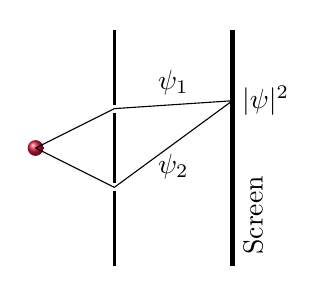
\begin{tikzpicture}
          \draw [very thick] (0,1.5) -- (0,.55) (0,.45) -- (0,-.45)
                             (0,-.55) -- (0,-1.5);
          \shade [ball color = Crimson] (-1,0) circle (.1);
          \draw (-1,0) -- (0,.5) -- (1.5,.6)
           node [midway, above] {$\psi_1$}
           (-1,0) -- (0,-.5) -- (1.5,.6) node [right] {$|\psi|^2$}
           node [midway, below] {$\psi_2$};
          \draw [ultra thick] (1.5,1.5) -- (1.5,-1.5)
           node [above right] {\rotatebox{90}{Screen}};
      \end{tikzpicture}
      \end{center}
      \end{paracol}
      The last term represents the interference between the two paths
      and is responsible for the pattern.
    \end{enumext}
    \item Stern-Gerlach experiment.
    \paragraph{Experiment Description}
    \begin{paracol}{2}
      Silver atoms are heated in an oven, then some of them
      escape from a small hole in the oven. The silver atom beam goes through
      a collimator and is then subjected to an inhomogeneous magnetic field.
      \switchcolumn
      \begin{center}
      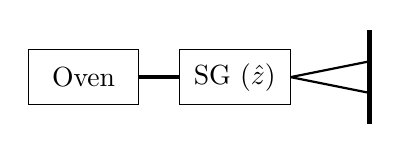
\begin{tikzpicture}
        \node [draw, minimum width = 4em, minimum height = 2em]
          (oven) at (0,0) {Oven};
        \node [draw, minimum width = 4em, minimum height = 2em, right = .5cm]
          (SG) at (oven.east) {SG ($\hat{\bm z}$)};
        \draw [very thick] (oven.east) -- (SG.west);
        \draw [thick] (SG.east) --++ (1,.2);
        \draw [thick] (SG.east) --++ (1,-.2);
        \draw [ultra thick] ([xshift = 1cm, yshift = .6cm]SG.east) --++
          (0,-1.2);
      \end{tikzpicture}
      \end{center}
    \end{paracol}
    Since the atoms in the oven are randomly oriented, people expect a continuous bundle of beams to come out of the magnetic field in the Stern-Gerlach apparatus.
    However, what the experiment observed is that the SG apparatus \emph{splits the original silver beam} from the oven \emph{into two distinct components}.
    \paragraph{Interpretation}
    The discrete deflection reveals that the electron spin is quantized.
    The magnetic moment of electrons (and thus atoms)
    can only take discrete values relative to any measurement axis.
    For electrons, the measurement of the spin component
    along any axis yields only one of two possible values:
    $+\hbar/2$ (spin up) or $-\hbar/2$ (spin down).
    \item Aharonov-Bohm effect.
    \paragraph{Experiment Description}
    \begin{paracol}{2}
      A beam of electrons is split into two paths
      (e.g., using a double-slit setup) that encircle a region
      containing a long solenoid that produces a confined magnetic field.
      The magnetic field $\bm B$ is zero outside the solenoid,
      but the magnetic vector potential $\bm A$ is non-zero outside.
      The two beams are recombined to produce interference fringes on a screen.
      \switchcolumn
      \begin{center}
        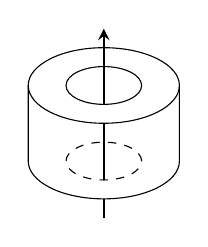
\begin{tikzpicture}[scale = .6]
          \draw (0,0) ellipse (1.6 and .8) ellipse (.8 and .4);
          \draw (-1.6,0) --++ (0,-1.6) arc (-180:0:1.6 and .8) --++ (0,1.6);
          \draw [dashed] (0,-1.6) ellipse (.8 and .4);
          \draw [thick] (0,-2.8) --++ (0,.4);
          \draw [thick] (0,-2) --++ (0,1.2);
          \draw [thick, -stealth] (0,-.4) --++ (0,1.6);
        \end{tikzpicture}
      \end{center}
    \end{paracol}

    When a current is passed through the solenoid,
    creating a magnetic flux $\Phi$ inside it,
    the interference pattern shifts \emph{even though
    the electrons travel in regions where the magnetic field is zero}.
    \paragraph{Interpretation}
    The effect highlights the non-local nature of quantum mechanics:
    electrons are influenced by the vector potential
    without entering the magnetic field region.
    The measured phase shift is gauge-invariant,
    depending on the enclosed magnetic flux,
    not the non-measurable potential itself.
  \end{enumext}
\end{solution}

% \clearpage

\begin{problem}[Optional, 30']
  Solve the hydrogen atom model:
  \[
    \mathcal H = \frac{\hat p^2}{2m} - \frac{e^2}{4 \pi \varepsilon_0} \frac1r.
  \]
\end{problem}
\begin{solution}
  Assume the wave function of hydrogen atom is
  $\Psi(r,t) = \psi(r) \upe^{-\iu\omega t}$.
  Substitute the time-independent wave function to Schr\"odinger equation
  \[
    \ab(-\frac{\hbar^2}{2m} \nabla^2 - \frac{e^2}{4\pi\varepsilon_0} \frac1r)
    \psi(r,\theta,\phi) = E \psi(r,\theta,\phi).
  \]
  Since the given hydrogen atom's potential is central,
  that is depends only on $r$, the Laplacian operator becomes
  \[
    \nabla^2 = \frac1{r^2} \pdv*{r^2 \pdv*{}r}r
             + \frac1{r^2\sin\theta} \pdv*{\sin\theta \pdv*{}\theta}\theta
             + \frac1{r^2\sin^2\theta} \pdv*[2]{}\phi.
  \]
  Referring to \emph{Mathematical Methods in Physics}, we have
  \[
    \ab(\frac1{\sin\theta} \pdv*{}\theta \sin\theta \pdv*{}\theta
  + \frac1{\sin^2\theta} \pdv*[2]{}\phi) Y_{lm}(\theta,\phi)
  = -l(l + 1) Y_{lm}(\theta,\phi).
  \]
  then we can separate the variables again. Let
  \[
    \psi(r,\theta,\phi) = R_{nl}(r) Y_{lm}(\theta,\phi),
  \]
  where $R_l(r)$ is the \emph{Radial Wave Function},
  and $Y_{lm}(\theta,\phi)$ is the spherical function. 
  Substitute $\psi(r,\theta,\phi)$ to Schr\"odinger equation, we have
  \[
    -\frac{\hbar^2}{2m} \frac1{r^2} \odv*{\ab(r^2 \odv{R_{nl}(r)}r)}r
    + \frac{\hbar^2 l (l + 1)}{2mr^2}R_{nl}(r)
    - \frac{e^2}{4\pi\varepsilon_0r} R_{nl}(r).
  \]
  Let $R_{nl}(r) = \chi_l(r)/r$, then substitute it to the Schr\"odinger equation,
  \[
    \chi''(r) + \ab[\frac{2m}{\hbar^2}\ab(E + \frac{e^2}{4\pi\varepsilon_0r})
    - \frac{l(l + 1)}{r^2}] \chi_l(r) = 0.
  \]
  To solve it, consider its asymptotic behavior first.
  \begin{enumext}[label = \roman*]
    \item When $r \to 0$, we have
    \[
      \chi_l''(r) - \frac{l(l+1)}{r^2} \chi_l(r) = 0.
    \]
    and we take the solution $\chi_l^0(r) = r^{l+1}$
    ($\chi_l^0(r) = r^{-l}$ is discard to avoid divergent).
    \item When $r \to \infty$, we have
    \[
      \chi_l''(r) + \frac{2m}{\hbar^2} E\chi_l(r) = 0
    \]
    and we take the solution $\chi_l^\infty(r) = \upe^{-kr}$,
    where $k = \sqrt{2mE/\hbar^2}$
    ($\chi_l^\infty(r) = \upe^{kr}$ is also discard).
  \end{enumext}
  To obtain the general solution, let
  \[
    \chi_l(r) = \chi_l^0(r) \chi_l^\infty(r) u_l(r).
  \]
  and substitute it to the Schr\"odinger equation
  \[
    \xi^2 \odv[2]{u_l(\xi)}\xi + [2(l + 1) - \xi] \odv{u_l(\xi)}\xi
  - \frac{2(L + 1)k - \frac{2me^2}{4\pi\varepsilon_0\hbar^2}}{2k} u_l(\xi) = 0,
  \]
  which suits the Laguerre polynomial
  \[
    \xi \odv[2]{u_l(\xi)}\xi + (\gamma - \xi) \odv{u_l(\xi)}\xi
  - \alpha u_l(\xi) = 0,
  \]
  compare with it, we have
  \[
    \gamma = 2(l + 1), \qq{and}
    \alpha = l + 1 - \frac{me^2}{4\pi\varepsilon_0 k\hbar^2}.
  \]
  Since the solution of this equation at $\xi = 0$ can be expanded into
  a series
  \[
    F_{\gamma,\alpha}(\xi)
  = 1 + \sum_{n = 1}^\infty\ab\{
    \ab[\frac{(\alpha + n - 1)!}{(\alpha - 1)!}\xi^n]\bigg/
    \ab[\frac{(\gamma + n - 1)!}{(\gamma - 1)!}n]\}.
  \]
  Apply \emph{d'Alembert's Judgement} to the $n$th
  and the $n + 1$th terms of $F_{\gamma,\alpha}(\xi)$
  \[
    \lim_{n\to\infty} \frac{f_{n+1}(\xi)}{f_n(\xi)} = \frac\xi n,
  \]
  means that $F_{\gamma,\alpha}(\xi)$ will divergent.
  To avoid this,
  the series needs to be cut off at the $n'$th term ($n'$ is finite), let
  $n' = -\alpha$, that is
  \[
    l + 1 - \frac{me^2}{4\pi\varepsilon_0 k\hbar^2} = n', \quad
    n \equiv l + 1 + n' = \frac{me^2}{4\pi\varepsilon_0 k\hbar^2},
  \]
  since $k = \sqrt{2mE/\hbar^2}$, we obtain the energy of hydrogen atom
  \[
    E_n = - \frac{me^4}{32\pi\varepsilon_0\hbar^2} \frac1{n^2}
  = -\frac{E_0}{n^2},
  \]
  and the basic state wave function is
  \[
    \psi_{100}(r,\theta,\phi) = \frac1{\sqrt{\pi a_0^3}} \upe^{-r/a_0}.
  \]
  where $a_0 = 4\pi\varepsilon_0\hbar^2/me^2$ is Bohr radius.
\end{solution}
